\documentclass{article}

\usepackage[margin=1in]{geometry}
\usepackage{tikz}
\usetikzlibrary{arrows.meta, positioning, fit, calc}

\begin{document}

\noindent\makebox[\textwidth][c]{%

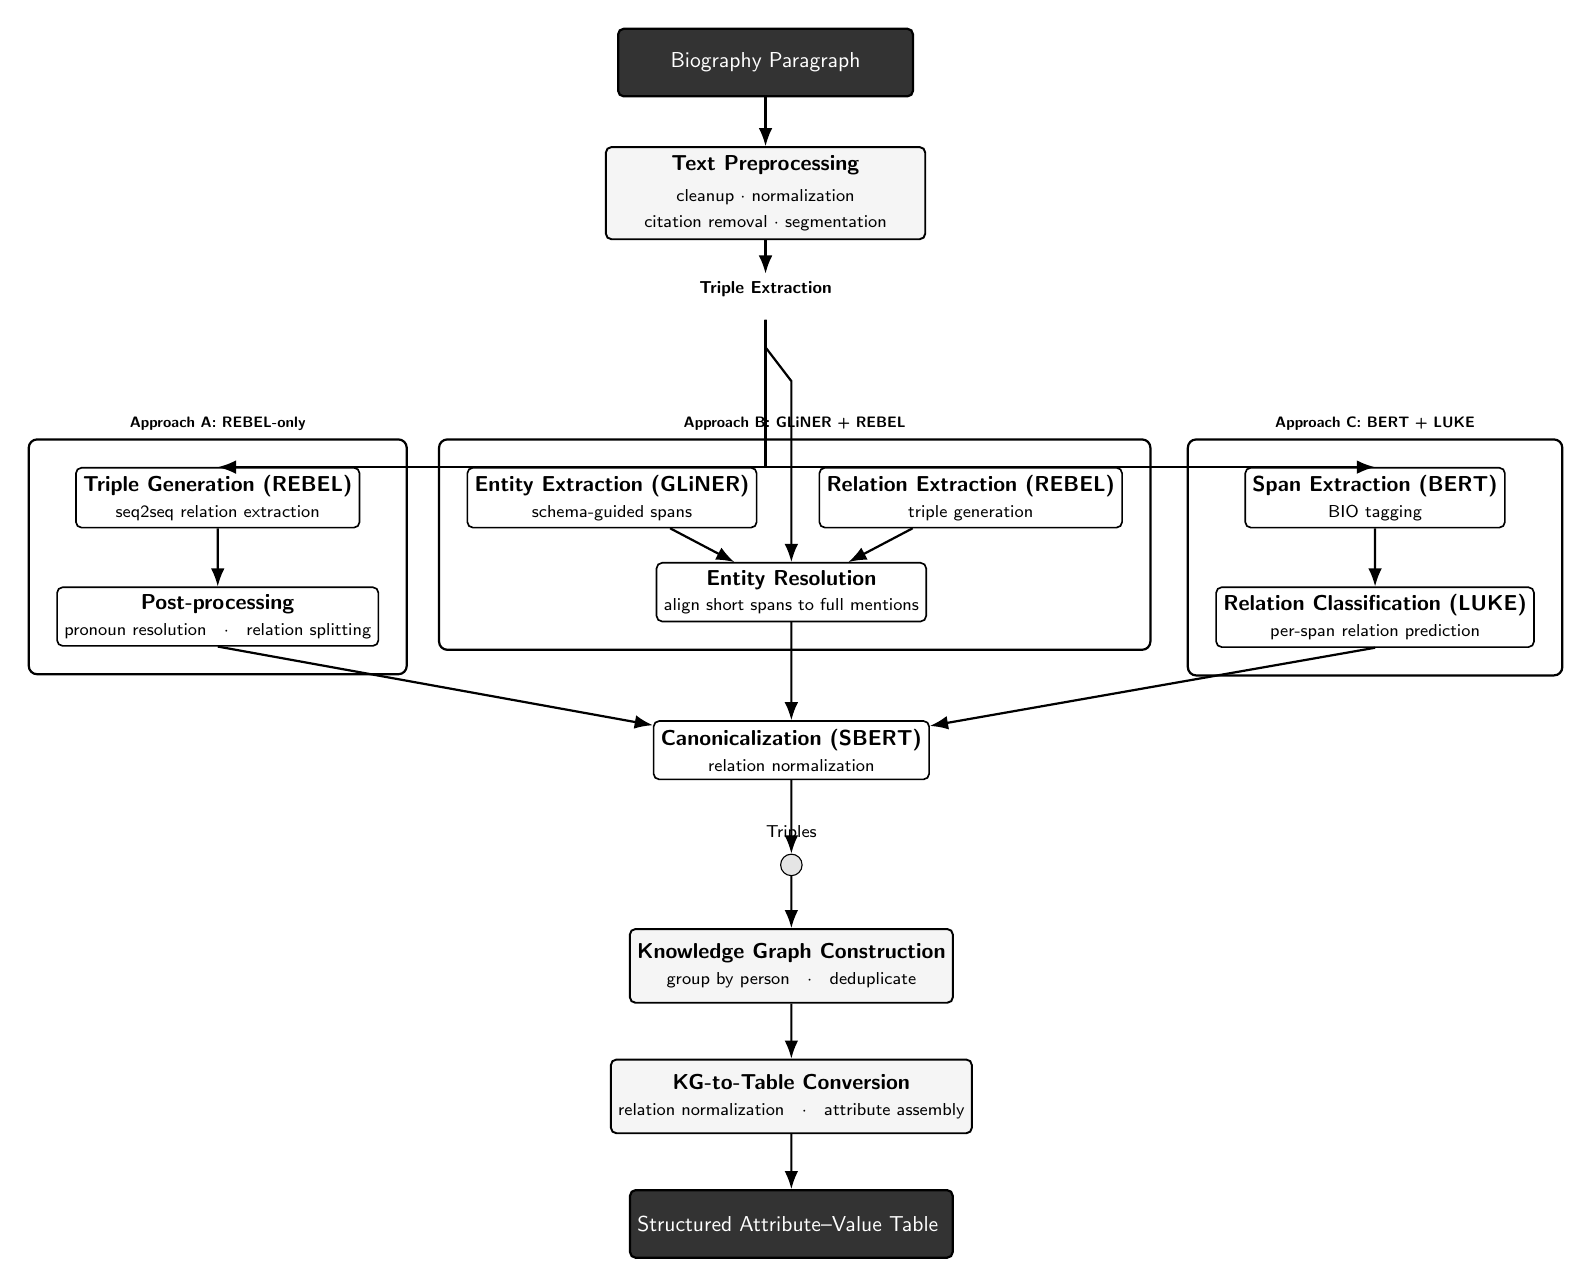
\begin{tikzpicture}[scale=0.78, transform shape,
    font=\sffamily,
    >=Latex,
    node distance=0.8cm,
    mainblock/.style={
        draw,
        rounded corners=2pt,
        minimum width=4.2cm,
        minimum height=1.0cm,
        align=center,
        fill=gray!8,
        line width=0.7pt
    },
    outputblock/.style={
        draw,
        rounded corners=2pt,
        minimum width=4.6cm,
        minimum height=1.1cm,
        align=center,
        fill=black!80,
        text=white,
        line width=0.8pt
    },
    innerblock/.style={
        draw,
        rounded corners=2pt,
        minimum width=3.4cm,
        minimum height=0.95cm,
        align=center,
        fill=white,
        line width=0.6pt
    },
    panel/.style={
        draw,
        rounded corners=3pt,
        inner sep=10pt,
        line width=0.8pt
    },
    flow/.style={
        ->,
        line width=0.8pt
    },
    smalltxt/.style={
        font=\sffamily\footnotesize,
        align=center
    }
]

% =====================
% Top shared pipeline
% =====================

\node[outputblock, minimum width=4.8cm] (input) {Biography Paragraph};

\node[mainblock, below=of input, minimum width=5.2cm, minimum height=1.5cm] (prep) {
    \textbf{Text Preprocessing}\\[2pt]
    {\footnotesize cleanup $\cdot$ normalization}\\
    {\footnotesize citation removal $\cdot$ segmentation}
};

\node[smalltxt, below=0.55cm of prep] (triplelabel) {\textbf{Triple Extraction}};

\draw[flow] (input) -- (prep);
\draw[flow] (prep) -- (triplelabel);

% Split point
\coordinate (split) at ($(triplelabel.south)+(0,-0.25)$);

% =====================
% Approach A
% =====================

\node[innerblock, below left=2.4cm and 6.6cm of split] (a1) {
    \textbf{Triple Generation (REBEL)}\\
    {\footnotesize seq2seq relation extraction}
};

\node[innerblock, below=0.95cm of a1] (a2) {
    \textbf{Post-processing}\\
    {\footnotesize pronoun resolution \; $\cdot$ \; relation splitting}
};

\node[panel, fit=(a1)(a2), label={[font=\sffamily\scriptsize\bfseries]north:Approach A: REBEL-only}] (A) {};

\draw[flow] (a1) -- (a2);

% =====================
% Approach B
% =====================

\node[innerblock, below=2.4cm of split, xshift=-2.5cm] (b1) {
    \textbf{Entity Extraction (GLiNER)}\\
    {\footnotesize schema-guided spans}
};

\node[innerblock, right=1.0cm of b1] (b2) {
    \textbf{Relation Extraction (REBEL)}\\
    {\footnotesize triple generation}
};

\node[innerblock, below=1.05cm of $(b1)!0.5!(b2)$, minimum width=3.4cm] (b3) {
    \textbf{Entity Resolution}\\
    {\footnotesize align short spans to full mentions}
};

\node[panel, fit=(b1)(b2)(b3), label={[font=\sffamily\scriptsize\bfseries]north:Approach B: GLiNER + REBEL}] (B) {};

\draw[flow] (b1) -- (b3);
\draw[flow] (b2) -- (b3);

% =====================
% Approach C
% =====================

\node[innerblock, below right=2.4cm and 7.8cm of split] (c1) {
    \textbf{Span Extraction (BERT)}\\
    {\footnotesize BIO tagging}
};

\node[innerblock, below=0.95cm of c1] (c2) {
    \textbf{Relation Classification (LUKE)}\\
    {\footnotesize per-span relation prediction}
};

\node[panel, fit=(c1)(c2), label={[font=\sffamily\scriptsize\bfseries]north:Approach C: BERT + LUKE}] (C) {};

\draw[flow] (c1) -- (c2);

% =====================
% Branch arrows from shared stage
% =====================

\draw[flow] (split) |- (a1.north);
\draw[flow] (split) -- ($(split)+(0,-0.45)$) -- ($(b3.north |- split)+(0,-1.0)$) -- (b3.north);
\draw[flow] (split) |- (c1.north);

% =====================
% Shared canonicalization
% =====================

\node[innerblock, below=1.6cm of b3, minimum width=3.6cm] (canon) {
    \textbf{Canonicalization (SBERT)}\\
    {\footnotesize relation normalization}
};

\draw[flow] (a2.south) -- (canon);
\draw[flow] (b3.south) -- (canon);
\draw[flow] (c2.south) -- (canon);

% =====================
% Merge point
% =====================

\node[draw, circle, fill=gray!20, minimum size=0.35cm, inner sep=0pt,
    below=1.2cm of canon] (merge) {};
\node[smalltxt, above=0.08cm of merge] {Triples};

\draw[flow] (canon) -- (merge);

% =====================
% Shared downstream
% =====================

\node[mainblock, below=0.85cm of merge, minimum width=4.8cm, minimum height=1.2cm] (kg) {
    \textbf{Knowledge Graph Construction}\\
    {\footnotesize group by person \; $\cdot$ \; deduplicate}
};

\node[mainblock, below=0.9cm of kg, minimum width=4.8cm, minimum height=1.2cm] (tableconv) {
    \textbf{KG-to-Table Conversion}\\
    {\footnotesize relation normalization \; $\cdot$ \; attribute assembly}
};

\node[outputblock, below=0.9cm of tableconv, minimum width=5.0cm] (output) {
    Structured Attribute--Value Table
};

\draw[flow] (merge) -- (kg);
\draw[flow] (kg) -- (tableconv);
\draw[flow] (tableconv) -- (output);

\end{tikzpicture}
}

\end{document}